\documentclass{beamer}


\usetheme{Warsaw}
\usecolortheme{crane}


\title{Solving Equations}
\subtitle{Mathematical Methods in the Physical Sciences}
\author{Steve Mazza}
\institute[Naval Postgraduate School]
{ 
    Naval Postgraduate School \\
    Monterey, CA \\
    
\includegraphics[height=3cm]{images/NPS_logo.jpg}
}
\date {SE3030, Winter/2014 \\ Quantitative Methods of Systems Engineering}
\subject{Quantitative Methods of Systems Engineering}


\begin{document}

\frame{\titlepage}


\frame{{Introduction}
	\begin{center}
		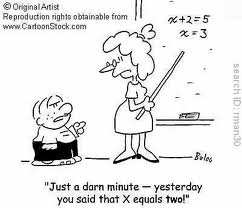
\includegraphics[scale=0.75]{images/algebraCartoon.jpg}
	\end{center}
}


\frame{{Solving an Equation in One Variable}
	Given an equation of the form $f(x)=0$, we want to find a solution to within the accuracy of our computations.
	We explore four methods
	\begin{itemize}
		\item Newton's Method, which uses a series of linear approximations by taking the derivative
		\item Poor Man's Newton, which uses a series of linear approximations without taking the derivative (numerical approximation).
		\item Another linear method that uses bracketing
		\item Divide and Conquer, which looks a little like a binary search
	\end{itemize}
}


\frame{{Newton's Method}
	\begin{block}{Newton-Raphson}
		\[x_{n+1} = x_n - \frac{f(n)}{f'(n)}\]
	\end{block}
	\begin{center}
		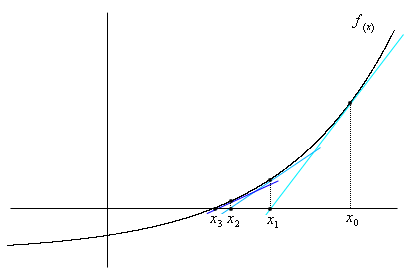
\includegraphics[scale=0.4]{images/newton_method_graph.png}
	\end{center}
	Geometrically, $(x_{n+1}, 0)$ is the intersection with the $x$-axis of the tangent to the graph of $f$ at $(x_n, f (x_n))$.
}


\frame{{Newton's Method Example}
	We calculate $\sqrt{5}$ by finding an approximate solution to the equation $f(x) = x^2-5 = 0$.  We choose a first approximation of $x_0=2$, so
	\begin{align*}
		f(x) &= x^2-5 \\
		f'(x) &= 2x \\
		fLx_0(x) &= f(x_0) + f'(x_0)(x-x_0) \\
		&= -1+4(x-2) \\
		&= 4x-9 = \frac{9}{4} = 2.25 \\
		fLx_1(x) &= f(x_1) + f'(x_1)(x-x_1) \\
		&= \left(\frac{81}{16}-5\right)+\frac{9}{2}\left(x-\frac{9}{4}\right) \\
		&= \frac{9}{2}x-\frac{161}{16} = 2.236111
	\end{align*}
}


\frame{{Newton's Method Caveats}
	\begin{itemize}
		\item Many functions have more than one zero
		\item Some functions will never converge
		\item Unfortunate initial guesses can be very misleading
		\item If $f$ is implicitly defined, we may find values for $x_n$ for which $f$ is undefined.
	\end{itemize}
	However, if $f$ goes from negative to positive at the true solution $x$, and $f'$ is increasing between $x$ and your guess $x_0$, which is greater than $x$, then the method will always converge.
}


\frame{{Poor Man's Newton}
	Instead of calculating the derivative at each successive step we use the following approximation
	\begin{block}{Approximation to the Derivative}
		\[f'(x) \approx \frac{f(x_i+d)-f(x_i)}{d}\]
	\end{block}
	Then in general,
	\begin{block}{Approximation to Newton}
		\[x_{n+1} = x_n-d\frac{f(x_n)}{f(x_n+d)-f(x_n)}\]
	\end{block}
	The trick is selecting an appropriate value for $d$.
}


\frame{{Another Linear Method}
	%TODO
}


\frame{{Divide and Conquer}
	%TODO
}


\frame{{Solving Two General Equations in Two Variables}
	%TODO
}

%TODO: Delete everything below here to the final frame.
%\frame{{Example of columns 1}
%    \begin{columns}[c]      % the "c" option specifies center vertical alignment
%    \column{.5\textwidth}   % column designated by a command
%     Contents of the first column
%    \column{.5\textwidth}
%     Contents split \\ into two lines
%    \end{columns}
%}

\frame{{Questions?}
	\begin{center}
		
\includegraphics[width=.7\textwidth]{images/fin.png}
	\end{center}
}

\end{document}
